% AUTO-GENERATED by build/gen_corpus.py from literature/corpus.tsv -- do not hand-edit.
\begin{figure}[t]
\centering
\definecolor{cc0}{HTML}{1F77B4}
\definecolor{cc1}{HTML}{FF7F0E}
\definecolor{cc2}{HTML}{2CA02C}
\definecolor{cc3}{HTML}{D62728}
\definecolor{cc4}{HTML}{9467BD}
\definecolor{cc5}{HTML}{8C564B}
\definecolor{cc6}{HTML}{E377C2}
\definecolor{cc7}{HTML}{17BECF}
\definecolor{cc8}{HTML}{BCBD22}
\definecolor{cc9}{HTML}{7F7F7F}
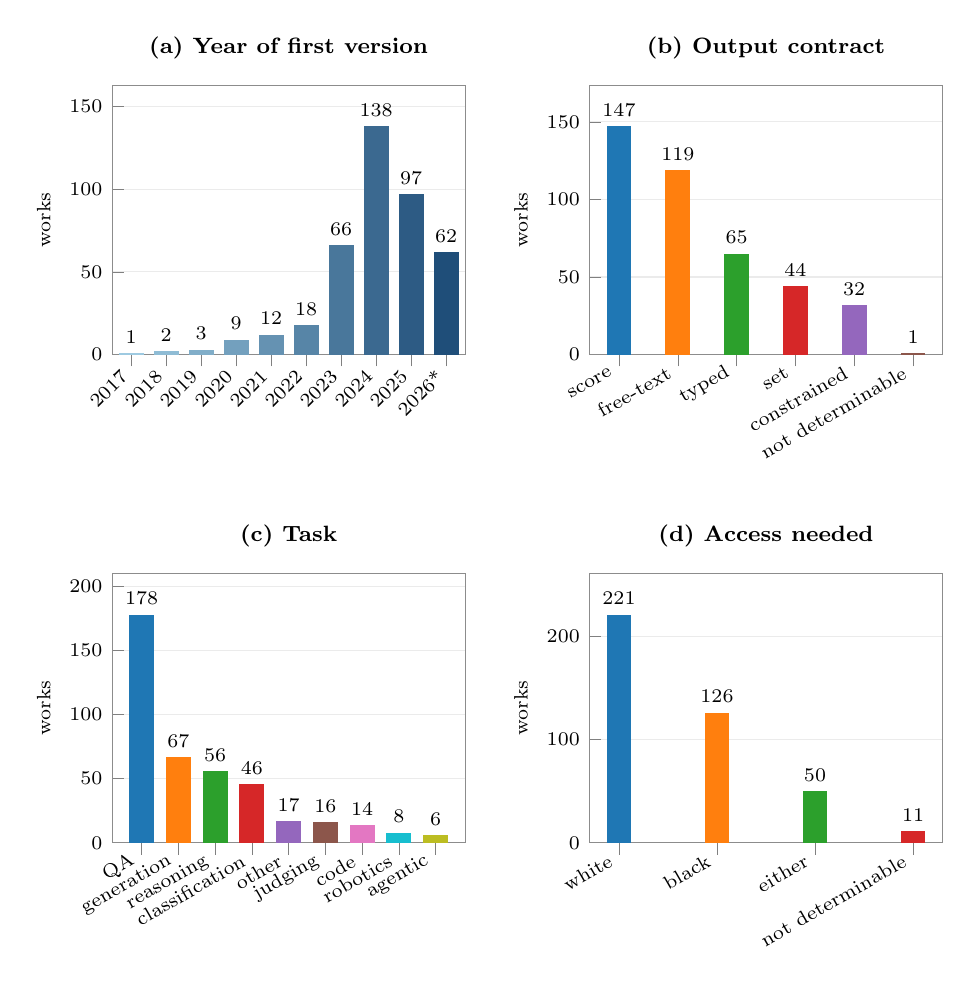
\begin{tikzpicture}
\begin{scope}\begin{axis}[ybar,bar width=9pt,width=0.5\textwidth,height=5cm,ymin=0,
  symbolic x coords={{2017},{2018},{2019},{2020},{2021},{2022},{2023},{2024},{2025},{2026*}},xtick={{2017},{2018},{2019},{2020},{2021},{2022},{2023},{2024},{2025},{2026*}},x tick label style={font=\scriptsize,rotate=45,anchor=east},
  nodes near coords,nodes near coords style={font=\scriptsize},title={\footnotesize\bfseries (a) Year of first version},
  ylabel={\scriptsize works},tick label style={font=\scriptsize},axis line style={black!45},tick pos=left,ymajorgrids,grid style={black!8},
  enlarge x limits=0.06,enlarge y limits={upper,value=0.18}]
\addplot[fill={rgb,255:red,158;green,202;blue,225},draw=none,bar shift=0pt] coordinates {({2017},1)};
\addplot[fill={rgb,255:red,143;green,188;blue,213},draw=none,bar shift=0pt] coordinates {({2018},2)};
\addplot[fill={rgb,255:red,129;green,174;blue,201},draw=none,bar shift=0pt] coordinates {({2019},3)};
\addplot[fill={rgb,255:red,115;green,160;blue,190},draw=none,bar shift=0pt] coordinates {({2020},9)};
\addplot[fill={rgb,255:red,101;green,146;blue,178},draw=none,bar shift=0pt] coordinates {({2021},12)};
\addplot[fill={rgb,255:red,87;green,133;blue,167},draw=none,bar shift=0pt] coordinates {({2022},18)};
\addplot[fill={rgb,255:red,73;green,119;blue,155},draw=none,bar shift=0pt] coordinates {({2023},66)};
\addplot[fill={rgb,255:red,59;green,105;blue,144},draw=none,bar shift=0pt] coordinates {({2024},138)};
\addplot[fill={rgb,255:red,45;green,91;blue,132},draw=none,bar shift=0pt] coordinates {({2025},97)};
\addplot[fill={rgb,255:red,31;green,78;blue,121},draw=none,bar shift=0pt] coordinates {({2026*},62)};
\end{axis}\end{scope}
\begin{scope}[xshift=0.5\textwidth]\begin{axis}[ybar,bar width=9pt,width=0.5\textwidth,height=5cm,ymin=0,
  symbolic x coords={{score},{free-text},{typed},{set},{constrained},{not determinable}},xtick={{score},{free-text},{typed},{set},{constrained},{not determinable}},x tick label style={font=\scriptsize,rotate=30,anchor=east},
  nodes near coords,nodes near coords style={font=\scriptsize},enlarge x limits=0.1,
  title={\footnotesize\bfseries (b) Output contract},ylabel={\scriptsize works},tick label style={font=\scriptsize},axis line style={black!45},tick pos=left,
  ymajorgrids,grid style={black!8},enlarge y limits={upper,value=0.18}]
\addplot[fill=cc0,draw=none,bar shift=0pt] coordinates {({score},147)};
\addplot[fill=cc1,draw=none,bar shift=0pt] coordinates {({free-text},119)};
\addplot[fill=cc2,draw=none,bar shift=0pt] coordinates {({typed},65)};
\addplot[fill=cc3,draw=none,bar shift=0pt] coordinates {({set},44)};
\addplot[fill=cc4,draw=none,bar shift=0pt] coordinates {({constrained},32)};
\addplot[fill=cc5,draw=none,bar shift=0pt] coordinates {({not determinable},1)};
\end{axis}\end{scope}
\begin{scope}[yshift=-6.2cm]\begin{axis}[ybar,bar width=9pt,width=0.5\textwidth,height=5cm,ymin=0,
  symbolic x coords={{QA},{generation},{reasoning},{classification},{other},{judging},{code},{robotics},{agentic}},xtick={{QA},{generation},{reasoning},{classification},{other},{judging},{code},{robotics},{agentic}},x tick label style={font=\scriptsize,rotate=30,anchor=east},
  nodes near coords,nodes near coords style={font=\scriptsize},enlarge x limits=0.1,
  title={\footnotesize\bfseries (c) Task},ylabel={\scriptsize works},tick label style={font=\scriptsize},axis line style={black!45},tick pos=left,
  ymajorgrids,grid style={black!8},enlarge y limits={upper,value=0.18}]
\addplot[fill=cc0,draw=none,bar shift=0pt] coordinates {({QA},178)};
\addplot[fill=cc1,draw=none,bar shift=0pt] coordinates {({generation},67)};
\addplot[fill=cc2,draw=none,bar shift=0pt] coordinates {({reasoning},56)};
\addplot[fill=cc3,draw=none,bar shift=0pt] coordinates {({classification},46)};
\addplot[fill=cc4,draw=none,bar shift=0pt] coordinates {({other},17)};
\addplot[fill=cc5,draw=none,bar shift=0pt] coordinates {({judging},16)};
\addplot[fill=cc6,draw=none,bar shift=0pt] coordinates {({code},14)};
\addplot[fill=cc7,draw=none,bar shift=0pt] coordinates {({robotics},8)};
\addplot[fill=cc8,draw=none,bar shift=0pt] coordinates {({agentic},6)};
\end{axis}\end{scope}
\begin{scope}[xshift=0.5\textwidth,yshift=-6.2cm]\begin{axis}[ybar,bar width=9pt,width=0.5\textwidth,height=5cm,ymin=0,
  symbolic x coords={{white},{black},{either},{not determinable}},xtick={{white},{black},{either},{not determinable}},x tick label style={font=\scriptsize,rotate=30,anchor=east},
  nodes near coords,nodes near coords style={font=\scriptsize},enlarge x limits=0.1,
  title={\footnotesize\bfseries (d) Access needed},ylabel={\scriptsize works},tick label style={font=\scriptsize},axis line style={black!45},tick pos=left,
  ymajorgrids,grid style={black!8},enlarge y limits={upper,value=0.18}]
\addplot[fill=cc0,draw=none,bar shift=0pt] coordinates {({white},221)};
\addplot[fill=cc1,draw=none,bar shift=0pt] coordinates {({black},126)};
\addplot[fill=cc2,draw=none,bar shift=0pt] coordinates {({either},50)};
\addplot[fill=cc3,draw=none,bar shift=0pt] coordinates {({not determinable},11)};
\end{axis}\end{scope}
\end{tikzpicture}
\caption{\textbf{Profile of the 408 corpus works} (Tables~\ref{tab:compare_s4} and~\ref{tab:landscape}). (a)~Year of first public version
(*2026 is partial); (b)~the output contract the confidence is attached to (the five contracts are defined in the caption of Table~\ref{tab:landscape}); (c)~task; (d)~the access a method needs:
white-box (logits or weights), black-box (text only) or either. ``not determinable'' marks a value that could not be determined from the paper.}
\Description{Four bar charts describing the corpus: works per year, per output contract, per task and per access level.}
\label{fig:corpus_dist}
\end{figure}
